\section{Peak Calling}
\textbf{Genom:}\\

\includegraphics[scale=0.5]{lectures/160415/pix/Peak1.png}
\\\\
Ergebnis: Sequenziertes Genom/RNA/DNA aus dem Experiment = viele, kurze Reads\\\\
\textbf{Frage:} Wo sind die Proteine gebunden?\\

3 Ansätze:
\begin{enumerate}
	\item naiver Ansatz: Jedes Nukleotid, dass durch mind. Read bedeckt ist, war gebunden $\Rightarrow$ viele False Positives, da kurze Reads mehrere Treffer haben können
	\item Cut off x: mind. x Reads müssen auf das Nukleotid gemappt sein $\Rightarrow$ Problem durch sequence bias: Manche Basen einfach zu binden = viele FP
	\item enrichment: $log\frac{Expression}{Background}$
\end{enumerate}

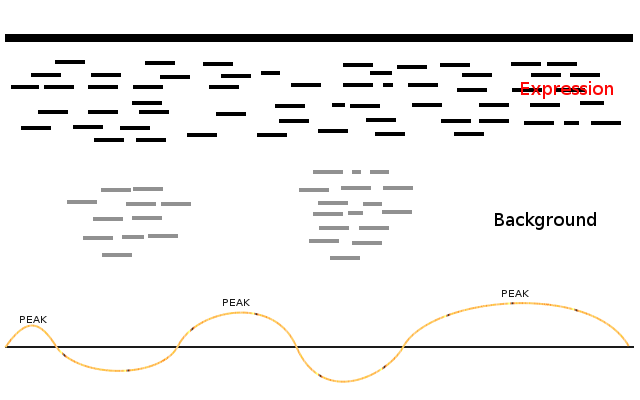
\includegraphics[scale=0.5]{lectures/160415/pix/Peak3.png}

naiv: Wenn Enrichtment $>$ Cutoff $\rightarrow$ Peak!
\\\\
\textbf{$\Rightarrow$ daher Entwicklung Peak Calling}\footnote{\url{https://en.wikipedia.org/wiki/Peak_calling}}
 - häufig verwendete Software: MACS (Model-based Analysis of ChIP-Seq)\footnote{\url{http://liulab.dfci.harvard.edu/MACS/}}


\textbf{\underline{1. }}\\
Einteilen des Genoms in Bins (Eimer), n Bins werden Reads eingeordnet\\
Window: 200 BP und Offset von 1/4 der window size\\\\
\begin{center}
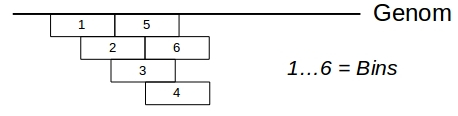
\includegraphics[scale=0.5]{lectures/160415/pix/sign.jpg}
\end{center}
\textbf{\underline{2. }}\\
Zählen der hypothetischen Fragmente pro Bin, +/- Strang\\
Ergebnis: Liste von Zahlen (Poisson verteilt!)
\begin{center}
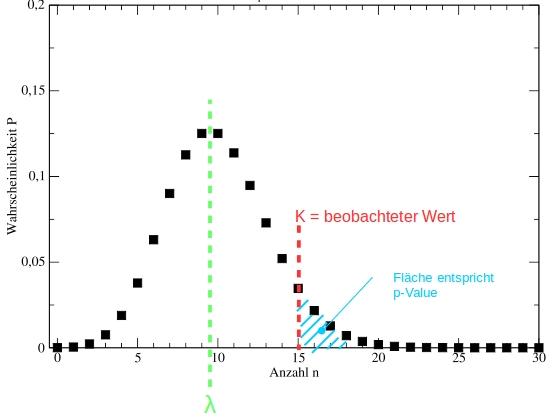
\includegraphics[scale=0.5]{lectures/160415/pix/poisson.jpg}
\end{center}
$\lambda$ (reelwertig) = Mittelwert der readcounts aus der Hintergrundmessung (Signal aus Experiment nicht zufällig verteilt, daher wird Hintergrund genutzt)\\
k= Anzahl der reads/fragments aus Experiment

$P(x \geq k|\lambda)=\sum \limits_{i=k}^{\infty}P\lambda(i)=\underbrace{1-\sum \limits_{i=0}^{k-1}P\lambda(i)}_{*}$
\\\\
es wird summiert statt integriert, da diskrete Verteilung\\
* Berechnung der Gegenwahrscheinlichkeit, da $\sum \limits_{i=k}^{\infty}$ schwer zu berechnen
\begin{equation}
P(x \geq k|\lambda)=1-\sum \limits_{n=0}^{k-1}\frac{\lambda^{n}}{n!}e^{-\lambda}
\end{equation}

P ist global, benötigt wird aber lokal\\
pro Bin werden 3 lokale + das globale verwendet (Vermeidung von lokalen Sequenzeffekten)
\\\\
$\lambda_{global}$ entspricht globalen Mittelwert
\\\\
$\lambda_{1k}, \lambda_{5k}, \lambda_{10k} \Rightarrow$ Mittel aller Bins in einem 1k, 5k oder 10k Window zentriert am entsprechenden Bin (K=1000)
\begin{center}
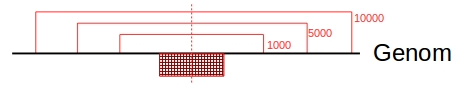
\includegraphics[scale=0.75]{lectures/160415/pix/lambdas.jpg}
\end{center}

$\lambda$=max($\lambda$global, $\lambda$1000, $\lambda$5000, $\lambda$10000)\\
neues $\lambda$ verschiebt Mittelwert der Verteilung nach rechts $\rightarrow$ k bleibt gleich $\rightarrow$ Wahrscheinlichkeit sinkt (keine Bias-Unterschätzung) $\rightarrow$ Reduzierung der False Positives
\\\\
da viele p-Values $\rightarrow$ multiple test problem
\\\\
\textbf{\underline{3. p-Value correction}}\\
 - bei MACS: Bonferroni-Holm (bleibt p-Value)\\
 - andere Möglichkeit: q-Value (Storeq) $\rightarrow$ kontrolliert False Discovery Rate\\
Ergebnis: Signifikanz pro Bin\\
\begin{center}
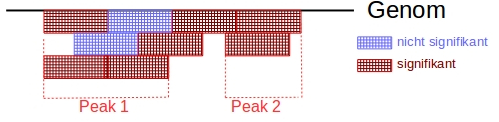
\includegraphics[scale=0.75]{lectures/160415/pix/sign2.jpg}
\end{center}
\textbf{\underline{4. Peakmerging}}\\
\begin{enumerate}
	\item bilden von Peaks über Bereiche von vielen signifikanten Bins
	\item Peak-Lücken vermeiden $\Rightarrow$ post processing, wenn Abstand zwischen Peaks $<$ Cutoff $\rightarrow$ Merge Peaks (bei MACS: cut-off=$ 2 \cdot $Bin-size)
\end{enumerate}
\textbf{
\underline{nächster Schritt: Vorhersage durch Motivs (Meme)}}\\

 - Wo sind die Bindungsstellen?
\\\\
\underline{CHIP-Seq:}\\
 - Region mit denen das Protein assoziiert ist (nicht wo es gebunden ist!)
\\\\
\underline{$\Rightarrow$ beide Informationen werden benötigt} - es werden immer Antikörper benötigt

\begin{enumerate}
	\item \textbf{Protein bekannt}, \textbf{gesucht ist RNA} welche vom Protein gebunden wird\\
	RIP: \underline{R}NA \underline{i}mmunoprecipitation \underline{p}rotocol (RIP-seq), Antikörper gegen Protein
	\item an welchen Stellen im Genom ist eine \textbf{RNA an eine DNA} gebunden?\\
	Chromatin extrahieren (ChIRP - seq: \underline{ch}romatin \underline{i}solation by \underline{R}NA \underline{p}urification), Antikörper gegen RNA oder komplementäres Lesen, DNA sequenzieren
\end{enumerate}

\underline{Problem:} nur Bereiche (Peaks) der Bindungen ermittelt, keine genauen Positionen
\begin{center}
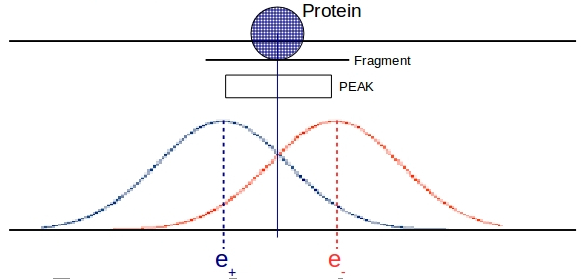
\includegraphics[scale=0.75]{lectures/160415/pix/result.jpg}
\end{center}
Erwartung: Peak sehr nah um das Protein\\
Mittelpunkt: e$_{+}$ und e$_{-}$ als Bindungstelle genommen